%! Author = TiagoRG
%! GitHub = https://github.com/TiagoRG

\documentclass{report}
\usepackage[T1]{fontenc} % Fontes T1
\usepackage[utf8]{inputenc} % Input UTF8
\usepackage[backend=biber, style=ieee]{biblatex} % para usar bibliografia
\usepackage{csquotes}
\usepackage[portuguese]{babel} %Usar língua portuguesa
\usepackage{blindtext} % Gerar texto automaticamente
\usepackage[dvipsnames]{xcolor}
\usepackage[printonlyused]{acronym}
\usepackage{hyperref} % para autoref
\usepackage{graphicx}
\usepackage{indentfirst}
\usepackage{float}
\usepackage{fancyhdr}
\usepackage{geometry}
\usepackage{listings}
\renewcommand{\familydefault}{\sfdefault}

\geometry{
    paper=a4paper,
    margin=45pt,
    % tmargin=70pt,
    includefoot
}

\lstset{
    language=C, % choose the language of the code
    basicstyle=\fontfamily{pcr}\selectfont\footnotesize\color{black},
    keywordstyle=\color{Blue}\bfseries, % style for keywords
    numbers=left, % where to put the line-numbers
    numberstyle=\tiny, % the size of the fonts that are used for the line-numbers
    backgroundcolor=\color{white},
    showspaces=false, % show spaces adding particular underscores
    showstringspaces=false, % underline spaces within strings
    showtabs=false, % show tabs within strings adding particular underscores
    frame=single, % adds a frame around the code
    tabsize=4, % sets default tabsize to 2 spaces
    rulesepcolor=\color{gray},
    rulecolor=\color{black},
    captionpos=b, % sets the caption-position to bottom
    breaklines=false, % sets automatic line breaking
    breakatwhitespace=false,
}

\bibliography{bibliography}


\begin{document}
%%
% Definições
%! Author = TiagoRG
%! GitHub = https://github.com/TiagoRG

\newcommand{\titulo}{Algoritmos e Estruturas de Dados\\
\vspace*{0.5cm}
1º Projeto}
\newcommand\data{DATA}
\newcommand\autores{Diogo Carvalho, Tiago Garcia}
\newcommand\autorescontactos{(113221) diogo.tav.carvalho@ua.pt, (114184) tiago.rgarcia@ua.pt}
\newcommand\departamento{Dept. de Eletrónica, Telecomunicações e Informática}
\newcommand\empresa{Universidade de Aveiro}

%
%%%%%% CAPA %%%%%%
%
\begin{titlepage}

\begin{center}
%
\vspace*{50mm}
%
{\Huge \titulo}\\
%
\vspace{10mm}
%
{\Large \empresa}\\
%
\vspace{10mm}
%
{\LARGE \autores}\\
%
\vspace{30mm}
%
\begin{figure}[h]
\center

\includegraphics{images/ua}\label{fig:ua-title-logo}
\end{figure}
%
\end{center}
\end{titlepage}

%%  Página de Título %%
\title{%
{\Huge\textbf{\titulo}}\\
\vspace*{1cm}
{\Large \departamento\\ \empresa}
}
%
\author{%
    \autores \\
    \autorescontactos
}
%
\date{\today}
%
\maketitle

%\pagenumbering{roman}

%%%%%% RESUMO %%%%%%
% \begin{abstract}
% Resumo de 200-300 palavras.
% \end{abstract}


%%%%%% Agradecimentos %%%%%%
%\renewcommand{\abstractname}{Agradecimentos}
%\begin{abstract}
    %Eventuais agradecimentos.
%\end{abstract}

\tableofcontents
%\listoftables     % descomentar se necessário
%\listoffigures    % descomentar se necessário


%%%%%%%%%%%%%%%%%%%%%%%%%%%%%%%
\clearpage

\renewcommand{\headrulewidth}{0pt}
\renewcommand{\footrulewidth}{0pt}
\fancypagestyle{plain}{
    \fancyhf{}% Clear header/footer
    % \fancyhead[R]{\small Universidade de Aveiro~~
\includegraphics[width=20pt,height=20pt]{images/ua}}% Right header
    % \fancyhead[L]{\small Departamento de Electrónica, Telecomunicações e Informática}% Right header
    \fancyfoot[C]{\thepage}% Centred footer
}
\pagestyle{plain}% Set page style to plain.

%%%%%% INTRODUÇÃO %%%%%%
%! Author = TiagoRG
%! GitHub = https://github.com/TiagoRG

\chapter{Introdução}
\label{ch:introducao}
{
%%%
% Conteúdo da introdução aqui

Neste projeto será desenvolvida uma ferramenta de manipulação de imagens monocromáticas (apenas um canal de cor, neste caso apenas escala de cinzentos), que permitirá efetuar diversas operações:

\begin{itemize}
    \item \textbf{ImageStats:} Mostra os valores mínimo e máximo dos pixeis da imagem;
    \item \textbf{ImageNegative:} Inverte os pixeis da imagem ($new\_value = max\_value - old\_value$);
    \item \textbf{ImageThreshold:} Aplica um limiar à imagem, de forma a que os pixeis com valor inferior ao limiar sejam convertidos para 0 e os restantes para o valor máximo;
    \item \textbf{ImageBrighten:} Aumenta ou diminui o brilho da imagem, multiplicando todos os pixeis por um fator ($fator~>~1$ aumenta o brilho, $fator~<~1$ diminui o brilho);
    \item \textbf{ImageMirror:} Espelha a imagem, horizontalmente;
    \item \textbf{ImageRotate:} Roda a imagem, 90º no sentido contrário ao dos ponteiros do relógio;
    \item \textbf{ImageCrop:} Corta a imagem, de acordo com as coordenadas do canto superior esquerdo e o tamanho do retângulo a cortar;
    \item \textbf{ImagePaste:} Cola uma imagem sobre outra a partir das coordenadas do canto superior esquerdo;
    \item \textbf{ImageBlend:} Cola uma imagem sobre outra, com um fator de transparência (entre 0 e 1), a partir das coordenadas do canto superior esquerdo;
    \item \textbf{ImageMatchSubImage:} Verifica se uma imagem está contida dentro de outra maior, a partir das coordenadas do canto superior esquerdo;
    \item \textbf{ImageLocateSubImage:} Procura uma imagem dentro de outra maior e devolve as coordenadas do canto superior esquerdo da primeira ocorrência;
    \item \textbf{ImageBlur:} Aplica um filtro de desfoque à imagem;
\end{itemize}

Tudo isto será desenvolvido usando a linguagem de programação C com recurso às bibliotecas stdio.h, stdlib.h, assert.h, ctype.h e errno.h.

\vspace{0.5cm}

Para as funções ImageLocateSubImage e ImageBlur será ainda feita a análise formal onde será apresentada a complexidade temporal e espacial de cada uma das funções. Para tal, será usada a notação O-grande, onde se considera apenas o termo de maior ordem. Será feita também uma análise experimental destas duas funções para verificar o resultado expectado pela análise formal. Por último, será descrito todo o algoritmo otimizado da função ImageBlur.

%%%
}



%%%%%%%%%%%%%%%%%%%%%%%%%%%%%%%%

% Capítulos
\chapter{ImageBlur}
\label{ch:imageblur}
\section{Análise formal}
\label{sec:imagelocatesubimage/formal}

\section{Análise formal}
\label{sec:imagelocatesubimage/formal}

\input{sec/imagematchsubimage/formal.tex}

\subsection{ImageLocateSubImage}

\subsubsection{Descrição do algoritmo}

A função ImageLocateSubImage compara uma imagem (img2) com uma imagem maior (img1). Após as verificações iniciais, percorre-se cada pixel da imagem, comparando-o com o da subimagem. Se for detetado um pixel igual, chama-se a função ImageMatchSubImage para verificar se a subimagem está presente na imagem maior. No caso de encontrar um pixel que não corresponda, a função continua até encontrar, ou até acabar a imagem. Caso a ImageMatchSubImage devolva verdadeiro, a função devolve verdadeiro.

\subsubsection{Análise de complexidade}

\begin{itemize}
    
\item
\textbf{Complexidade Temporal}

Sabemos que ImageMatchSubImage, presente dentro do loop interior, é uma operação $O(p*o)$, e que se percorre a imagem linha a linha e coluna a coluna, logo é possível afirmar que a complexidade temporal do algoritmo é $O((n*m)*(p*o))$, onde n e m são a altura e largura de img2 e p e o são a altura e largura da subimagem verificada dentro do loop, respetivamente.

\item
\textbf{Complexidade Espacial}

A complexidade espacial do algoritmo é $O(1)$, dado que não são usadas estruturas de dados adicionais que cresçam com o tamanho da entrada. As variáveis row e col são as únicas variáveis adicionais, e ocupam um espaço constante.

\end{itemize}


\subsection{ImageLocateSubImage}

\subsubsection{Descrição do algoritmo}

A função ImageLocateSubImage compara uma imagem (img2) com uma imagem maior (img1). Após as verificações iniciais, percorre-se cada pixel da imagem, comparando-o com o da subimagem. Se for detetado um pixel igual, chama-se a função ImageMatchSubImage para verificar se a subimagem está presente na imagem maior. No caso de encontrar um pixel que não corresponda, a função continua até encontrar, ou até acabar a imagem. Caso a ImageMatchSubImage devolva verdadeiro, a função devolve verdadeiro.

\subsubsection{Análise de complexidade}

\begin{itemize}
    
\item
\textbf{Complexidade Temporal}

Sabemos que ImageMatchSubImage, presente dentro do loop interior, é uma operação $O(p*o)$, e que se percorre a imagem linha a linha e coluna a coluna, logo é possível afirmar que a complexidade temporal do algoritmo é $O((n*m)*(p*o))$, onde n e m são a altura e largura de img2 e p e o são a altura e largura da subimagem verificada dentro do loop, respetivamente.

\item
\textbf{Complexidade Espacial}

A complexidade espacial do algoritmo é $O(1)$, dado que não são usadas estruturas de dados adicionais que cresçam com o tamanho da entrada. As variáveis row e col são as únicas variáveis adicionais, e ocupam um espaço constante.

\end{itemize}

\section{Análise experimental}
\label{sec:imagelocatesubimage/experimental}

WIP
\pagebreak
\section{Algoritmo optimizado da ImageBlur}
\label{sec:imageblur/optimal}

\subsection{Descrição do algoritmo}

Este algoritmo passa por calcular as somas todas recursivamente antes de começar a criar a imagem desfocada. Uma vez que teremos as somas todas calculadas, podemos calcular o valor de cada pixel da imagem desfocada com base nas somas calculadas anteriormente. Este algoritmo é mais eficiente que o anterior pois não temos de calcular as somas de cada pixel da imagem desfocada, mas sim apenas uma vez para cada pixel da imagem original.

\subsection{Implementação}

\subsubsection{Imagem Integral}

Considerando $img$ como uma matriz $m \times n$, onde $m~=~img\rightarrow height$ e $n~=~img\rightarrow width$, vamos gerar uma matriz $m+1 \times n+1$ onde a primeira linha e a primeira coluna vão ser zeros, a partir daí, o elemento $(y,x)$ desta matriz irá corresponder ao elemento $(y-1,x-1)$ da matriz da imagem com $x\in[1,n]$ e $y\in[1,m]$. Esta nova imagem será armazenada como um array de $m+1~*~n+1$ elementos, com 32 bits cada (visto que será um array de inteiros).

Para inicializar a matriz, usamos as linhas de código:

\begin{lstlisting}[language=C]
    int integral_width = img->width + 1;
    int integral_height = img->height + 1;
    int* integral = (int*)calloc(integral_width * integral_height, sizeof(int));
\end{lstlisting}

Agora vamos ter de completar o resto das células. Cada célula da nova matriz será igual à soma de todos os pixeis que estão acima e à esquerda do mesmo.

\begin{figure}[H]
    \centering
    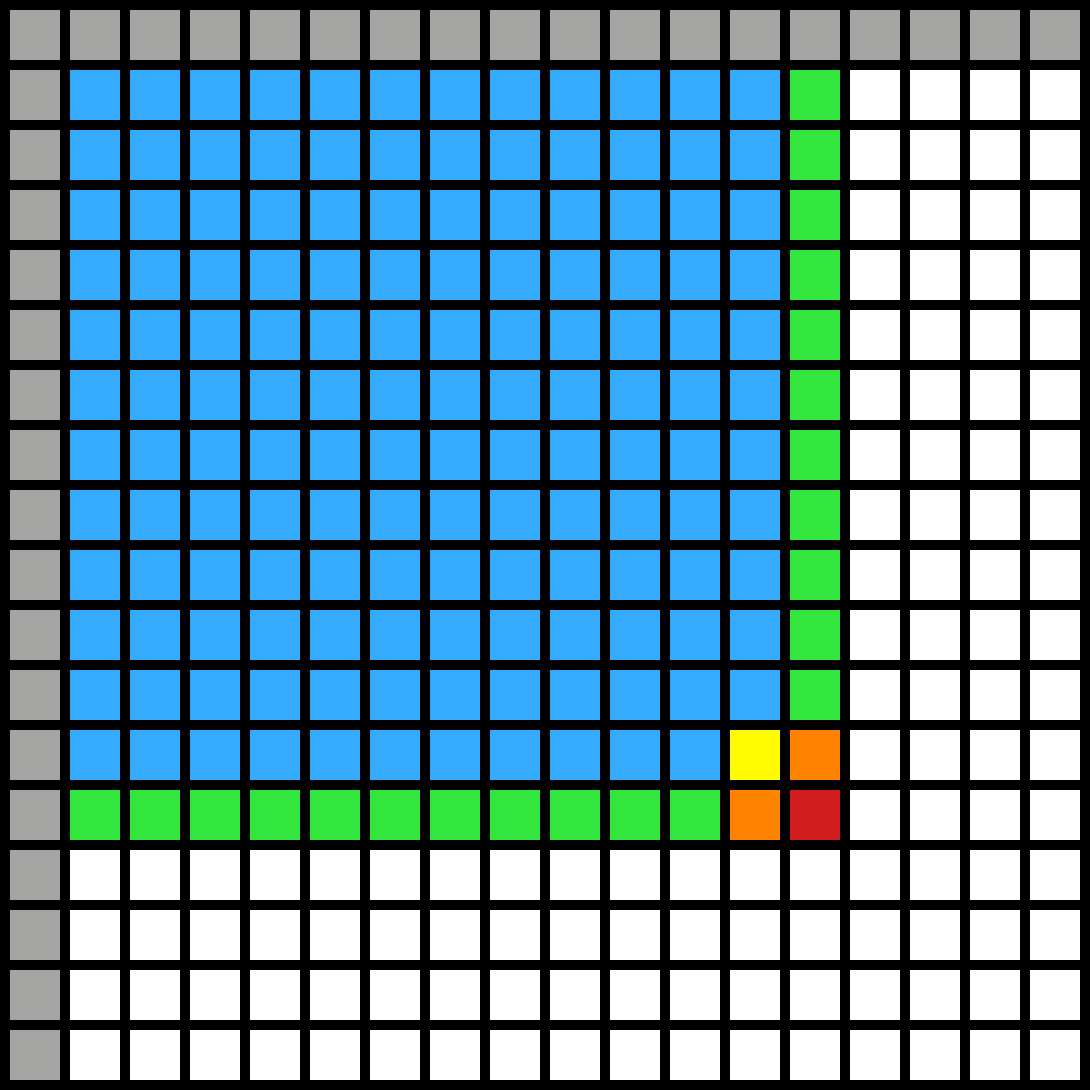
\includegraphics[width=0.4\linewidth]{images/integral-matrix.png}
    \caption{Representação da matriz integral}
\end{figure}

Como podemos ver na figura acima, para calcular o pixel representado a \textcolor{red}{\textbf{vermelho}} ($I_{(y,x)}$), teremos de adicionar ao pixel original da imagem, depois, o elemento representado acima a \textcolor{orange}{\textbf{laranja}} ($I_{(y-1,x)}$) que já contém todos os pixeis acima e à esquerda do mesmo (representados a \textcolor{green}{\textbf{verde}} acima do pixel mencionado), e por fim, teremos de adicionar o elemento representado à esquerda também a \textcolor{orange}{\textbf{laranja}} ($I_{(y, x-1)}$) que contém todos os pixeis na linha horizontal à esquerda do mesmo (representados a \textcolor{green}{\textbf{verde}} à esquerda do pixel mencionado). Uma vez que o pixel $I_{(y,x-1)}$, também contém a área acima dele (parte já incluída pelo pixel $I_{(y-1,x)}$), então teremos de remover a parte duplicada (área representada a \textcolor{blue}{\textbf{azul}}) que corresponde ao valor do pixel representado a \textcolor{yellow}{\textbf{amarelo}} ($I_{(y-1,x-1)}$). Com isto, podemos concluir que a expressão para cálcular a área a atribuir a um determinado pixel será:

\begin{equation}
    I_{(y,x)} = O_{(y-1,x-1)} + I_{(y-1,x)} + I_{(y,x-1)} - I_{(y-1,x-1)}
\end{equation}\label{eq:equacao-para-integral}

De notar que as células representadas a \textcolor{gray}{\textbf{cinzento}} serão as células cujo valor do elemento será sempre zero.

Para calcular todas estas células da matriz, usamos as linhas de código:

\begin{lstlisting}[language=C]
    for (int y = 1; y < integral_height; y++) {
        for (int x = 1; x < integral_width; x++) {
            integral[y * integral_width + x] = ImageGetPixel(img, x - 1, y - 1)   
                + integral[(y - 1) * integral_width + x]                          
                + integral[y * integral_width + (x - 1)]                          
                - integral[(y - 1) * integral_width + (x - 1)];                   
        }
    }
\end{lstlisting}

\subsubsection{Imagem desfocada}

Uma vez que já temos a imagem integral, podemos agora calcular a imagem desfocada. Para isso, vamos percorrer a imagem integral e para cada pixel, teremos de efetuar o seguinte procedimento:

\begin{enumerate}

\item {
\textbf{Calcular os cantos do retângulo de blur}

Vamos calcular a soma dos pixeis que estão dentro do retângulo de dimensões $2dx+1$ e $2dy+1$ para o comprimento e largura, respetivamente, centrado no pixel atual. Poderemos obter esse retângulo usando o canto superior esquerdo bem como o canto inferior direito.

\begin{enumerate}
    

    \item {
        \textbf{Canto superior esquerdo}

        Para obter cada uma das coordenadas deste ponto, teremos de subtrair a cada coordenada do pixel, os valores do $dy$ e $dx$, $dy$ para a borda superior e $dx$ para a borda da esquerda. No caso do resultado de uma dessas coordenadas ultrapassar um dos limites mínimos do retângulo, então esta coordenada deverá ser o limite mínimo. Este limite normalmente seria 0 mas visto que na imagem integral temos uma linha e uma coluna extra em cima e à esquerda, então temos de somar 1 a esses limites para compensar pelos pixeis extra e redefinir o início da parte útil da matriz. Isto fará que o limite mínimo seja 1 à esquerda e em cima. Para calcular as coordenadas, usamos as linhas de código: 

        \begin{lstlisting}[language=C]
int x1 = x - dx < 1 ? 1 : x - dx;
int y1 = y - dy < 1 ? 1 : y - dy;
        \end{lstlisting}
    }
    \item {
        \textbf{Canto inferior direito}

        Para obter cada uma das coordenadas deste ponto, teremos de somar a cada coordenada do pixel, os valores do $dy$ e $dx$, $dy$ para a borda inferior e $dx$ para a borda da direita. No caso do resultado de uma dessas coordenadas ultrapassar um dos limites máximos do retângulo, então esta coordenada deverá ser o limite máximo. Uma vez que deste lado não temos nenhuma linha ou coluna extra, o limite máximo será o último indice, ou seja, $integral\_width-1$. Isto fará que o limite máximo seja a largura menos 1 à direita e a altura menos 1 em baixo. Aos resultados, teremos de adicionar o valor 1 visto que não é contabilizada a linha/coluna do pixel central. Para calcular as coordenadas, usamos as linhas de código:

        \begin{lstlisting}[language=C]
int x2 = x + dx + 1 > integral_width - 1 ? integral_width - 1 : x + dx + 1;
int y2 = y + dy + 1 > integral_height - 1 ? integral_height - 1 : y + dy + 1;
        \end{lstlisting}
    }
\end{enumerate}
}

\pagebreak

\item {
\textbf{Cálculo da quantidade de pixeis}

Para calcular a quantidade de pixeis que estão dentro do retângulo, basta calcular a área do retângulo em pixeis, ou seja, a multiplicação do comprimento pela largura. Para tal, usamos a linha de código:

\begin{lstlisting}[language=C]
    int count = (x2 - x1) * (y2 - y1);
\end{lstlisting}
}

\item {
\textbf{Cálculo da soma}

\begin{figure}[H]
    \centering
    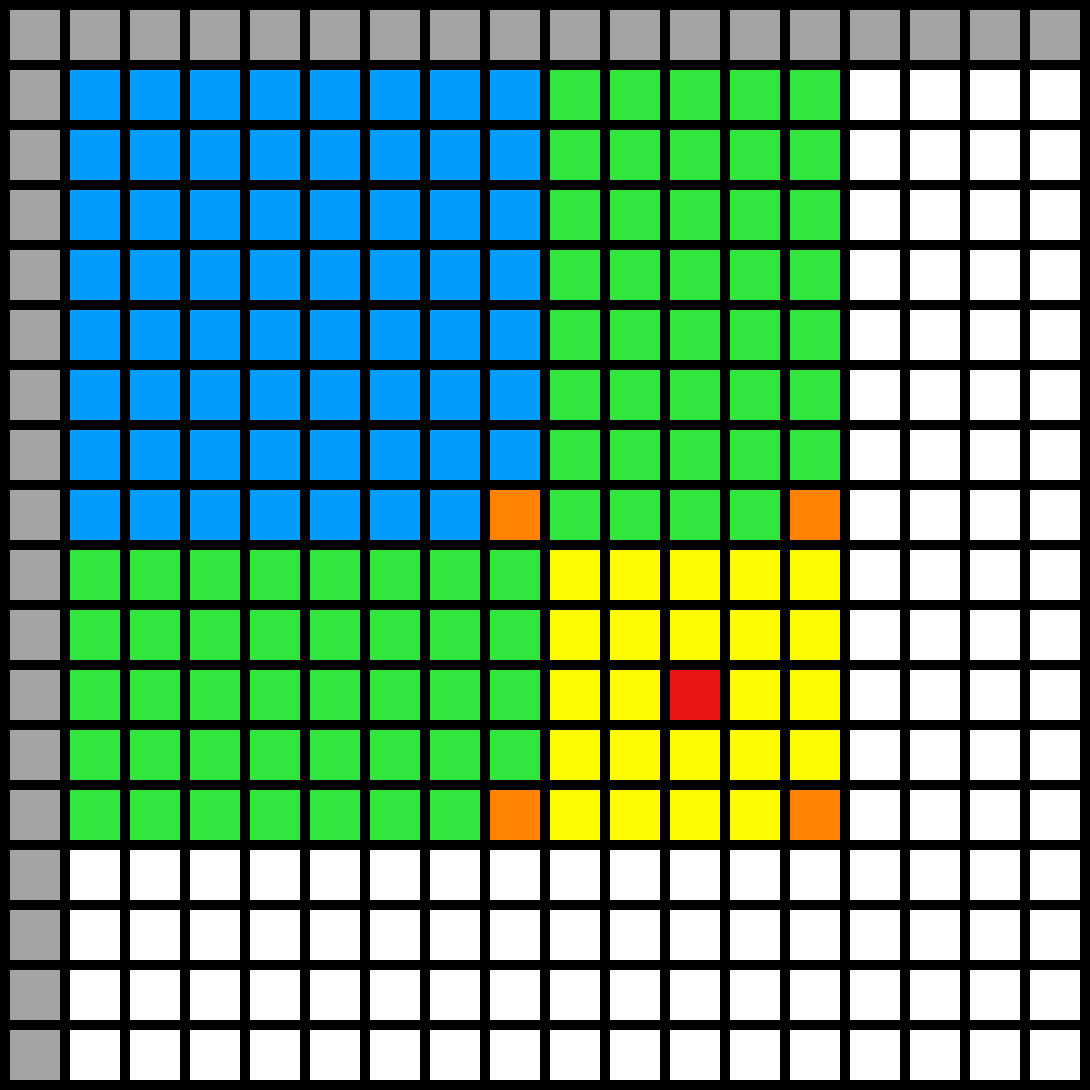
\includegraphics[width=0.4\linewidth]{images/rectangle-area.png}
    \caption{Representação do retângulo de blur}
\end{figure}

Como podemos ver pela figura anterior, para conseguir a área pretendidada (representada a \textcolor{yellow}{\textbf{amarelo}}), temos de usar como base a área associada ao pixel do canto inferior direito e subtrair a área associada ao pixel do canto superior direito (área acima do retângulo) bem como subtrair a área associada ao pixel do canto inferior esquerdo (área à esquerda do retângulo). Estas áreas exteriores ao retângulo estão representadas a \textcolor{green}{\textbf{verde}}. Visto que uma parte destas áreas coincide, temos de tirar a parte duplicada que será a área associada ao pixel do canto superior esquerdo e representada a \textcolor{blue}{\textbf{azul}} na imagem. Importante notar que enquanto que o canto inferior direito será incluído na área, os outros 3 cantos não serão. A partir disto, podemos obter a soma do retângulo de blur a partir da seguinte expressão:

\begin{equation}
    S_{(y,x)} = I_{(y2,x2)} - I_{(y1,x2)} - I_{(y2,x1)} + I_{(y1,x1)}
\end{equation}\label{eq:equacao-para-soma}

Para calcular o resultado desta expressão, usamos as linhas de código:

\begin{lstlisting}[language=C]
    int sum = integral[y2 * integral_width + x2]
        - integral[y1 * integral_width + x2]
        - integral[y2 * integral_width + x1]
        + integral[y1 * integral_width + x1];
\end{lstlisting}
}

\item {
\textbf{Definir o novo valor do pixel}

Para definir o novo valor do pixel, basta dividir a soma pelo número de pixeis que estão dentro do retângulo. Para tal, usamos a linha de código:

\begin{lstlisting}[language=C]
    ImageSetPixel(img, x, y, (sum + count / 2) / count);
\end{lstlisting}

De notar que somamos $count/2$ à soma para que o resultado da divisão seja arredondado corretamente.
}

Após repetir este procedimento para todos os pixeis da imagem, obtemos a imagem desfocada.
\end{enumerate}


\chapter{ImageMatchSubImage e ImageLocateSubImage}
\label{ch:imagematchlocatesubimage}
\section{Análise formal}
\label{sec:imagelocatesubimage/formal}

\section{Análise formal}
\label{sec:imagelocatesubimage/formal}

\input{sec/imagematchsubimage/formal.tex}

\subsection{ImageLocateSubImage}

\subsubsection{Descrição do algoritmo}

A função ImageLocateSubImage compara uma imagem (img2) com uma imagem maior (img1). Após as verificações iniciais, percorre-se cada pixel da imagem, comparando-o com o da subimagem. Se for detetado um pixel igual, chama-se a função ImageMatchSubImage para verificar se a subimagem está presente na imagem maior. No caso de encontrar um pixel que não corresponda, a função continua até encontrar, ou até acabar a imagem. Caso a ImageMatchSubImage devolva verdadeiro, a função devolve verdadeiro.

\subsubsection{Análise de complexidade}

\begin{itemize}
    
\item
\textbf{Complexidade Temporal}

Sabemos que ImageMatchSubImage, presente dentro do loop interior, é uma operação $O(p*o)$, e que se percorre a imagem linha a linha e coluna a coluna, logo é possível afirmar que a complexidade temporal do algoritmo é $O((n*m)*(p*o))$, onde n e m são a altura e largura de img2 e p e o são a altura e largura da subimagem verificada dentro do loop, respetivamente.

\item
\textbf{Complexidade Espacial}

A complexidade espacial do algoritmo é $O(1)$, dado que não são usadas estruturas de dados adicionais que cresçam com o tamanho da entrada. As variáveis row e col são as únicas variáveis adicionais, e ocupam um espaço constante.

\end{itemize}


\subsection{ImageLocateSubImage}

\subsubsection{Descrição do algoritmo}

A função ImageLocateSubImage compara uma imagem (img2) com uma imagem maior (img1). Após as verificações iniciais, percorre-se cada pixel da imagem, comparando-o com o da subimagem. Se for detetado um pixel igual, chama-se a função ImageMatchSubImage para verificar se a subimagem está presente na imagem maior. No caso de encontrar um pixel que não corresponda, a função continua até encontrar, ou até acabar a imagem. Caso a ImageMatchSubImage devolva verdadeiro, a função devolve verdadeiro.

\subsubsection{Análise de complexidade}

\begin{itemize}
    
\item
\textbf{Complexidade Temporal}

Sabemos que ImageMatchSubImage, presente dentro do loop interior, é uma operação $O(p*o)$, e que se percorre a imagem linha a linha e coluna a coluna, logo é possível afirmar que a complexidade temporal do algoritmo é $O((n*m)*(p*o))$, onde n e m são a altura e largura de img2 e p e o são a altura e largura da subimagem verificada dentro do loop, respetivamente.

\item
\textbf{Complexidade Espacial}

A complexidade espacial do algoritmo é $O(1)$, dado que não são usadas estruturas de dados adicionais que cresçam com o tamanho da entrada. As variáveis row e col são as únicas variáveis adicionais, e ocupam um espaço constante.

\end{itemize}

\section{Análise experimental}
\label{sec:imagelocatesubimage/experimental}

WIP

%%%%%% CONCLUSÕES %%%%%%
%! Author = TiagoRG
%! GitHub = https://github.com/TiagoRG

\chapter{Conclusões}
\label{ch:conclusoes}
{

Em conclusão, o trabalho desenvolvido permitiu-nos aprofundar os nossos conhecimentos na linguagem C, bem como aprofundar os nossos conhecimentos em algoritmos e na sua optimização. Testou as nossas capacidades de resolução de problemas e de trabalho em equipa, bem como a nossa capacidade de análise e de síntese, e serviu para demonstrar a importância de código optimizado.
Como tal, foram vistas inúmeras melhorias a nível da complexidade espacial e, especialmente, a nível da complexidade temporal, com impactos significativos no tempo de execução de certas funcionalidades.

}


%%%%%% ACRÓNIMOS %%%%%%
%%! Author = TiagoRG
%! GitHub = https://github.com/TiagoRG

\chapter*{Acrónimos}
\begin{acronym}
    \acro{deti}[DETI]{Departamento de Eletrónica, Telecomunicações e Informática}
    \acro{leci}[LECI]{Licenciatura em Engenharia de Computadores e Informática}
    \acro{ua}[UA]{Universidade de Aveiro}
\end{acronym}


%%%%%%%%%%%%%%%%%%%%%%%%%%%%%%%%%
%\printbibheading
%\printbibliography

\chapter{Anexos}
\label{ch:anexos}

\scriptsize

\section{ImageBlur: Primeira Abordagem}
\label{sec:anexos/blur1}

\begin{lstlisting}[language=C]
void ImageBlur(Image img, int dx, int dy) {
    assert(img != NULL);
    assert(dx >= 0 && dy >= 0);

    if (dx == 0 && dy == 0) return;

    Image img_new = ImageCreate(img->width, img->height, img->maxval);
    if (img_new == NULL) return;

    for (int x = 0; x < img->width; x++) {
        for (int y = 0; y < img->height; y++) {
            int sum = 0;
            int count = 0;

            for (int ix = x - dx; ix <= x + dx; ix++) {
                for (int iy = y - dy; iy <= y + dy; iy++) {
                    if (!ImageValidPos(img, ix, iy)) continue;
                    sum += ImageGetPixel(img, ix, iy);
                    count++;
                }
            }

            ImageSetPixel(img_new, x, y, (sum + count / 2) / count);
        }
    }

    uint8 *tmp = img->pixel;
    img->pixel = img_new->pixel;
    img_new->pixel = tmp;

    ImageDestroy(&img_new);
}
\end{lstlisting}

\pagebreak

\section{ImageBlur: Segunda Abordagem}
\label{sec:anexos/blur2}

\begin{lstlisting}[language=C]
void ImageBlur(Image img, int dx, int dy) {
    assert(img != NULL);
    assert(dx >= 0 && dy >= 0);

    if (dx == 0 && dy == 0) return;

    int integral_width = img->width + 1;
    int integral_height = img->height + 1;
    int* integral = (int*)calloc(integral_width * integral_height, sizeof(int));
    for (int y = 1; y < integral_height; y++) {
        for (int x = 1; x < integral_width; x++) {
            integral[y * integral_width + x] = ImageGetPixel(img, x - 1, y - 1)   
                + integral[(y - 1) * integral_width + x]                          
                + integral[y * integral_width + (x - 1)]                          
                - integral[(y - 1) * integral_width + (x - 1)];                   
        }
    }

    for (int y = 0; y < img->height; y++) {
        for (int x = 0; x < img->width; x++) {
            int x1 = x - dx < 1 ? 1 : x - dx;
            int y1 = y - dy < 1 ? 1 : y - dy;

            int x2 = x + dx + 1 > integral_width - 1 ? integral_width - 1 : x + dx + 1;
            int y2 = y + dy + 1 > integral_height - 1 ? integral_height - 1 : y + dy + 1;

            int count = (x2 - x1) * (y2 - y1);

            int sum = integral[y2 * integral_width + x2]
                - integral[y1 * integral_width + x2]
                - integral[y2 * integral_width + x1]
                + integral[y1 * integral_width + x1];

            ImageSetPixel(img, x, y, (sum + count / 2) / count);
        }
    }

    free(integral);
}
\end{lstlisting}


\end{document}
